\subsection{Applying the Algorithm to the Graph}\label{sec:apply}
We run Algorithm~\ref{alg:dc} on $G$ with the paper's shortest-bridge merge (Algorithm~\ref{alg:merge})
and random seed \DCSeed{}. Fixing the seed makes the random choices, and so the result, reproducible.

\paragraph{Divide.} Figure~\ref{fig:tree} shows the recursion. Each box is a subset of vertices together
with the axis chosen to split it. The leaves are the base cases: one vertex (length 0), or two vertices
$a\to b\to a$ (length $2w(a,b)$).

\begin{figure}[H]
\centering
\resizebox{\textwidth}{!}{% AUTO-GENERATED by code/main.py --export-latex. Do not edit; re-run the export instead.
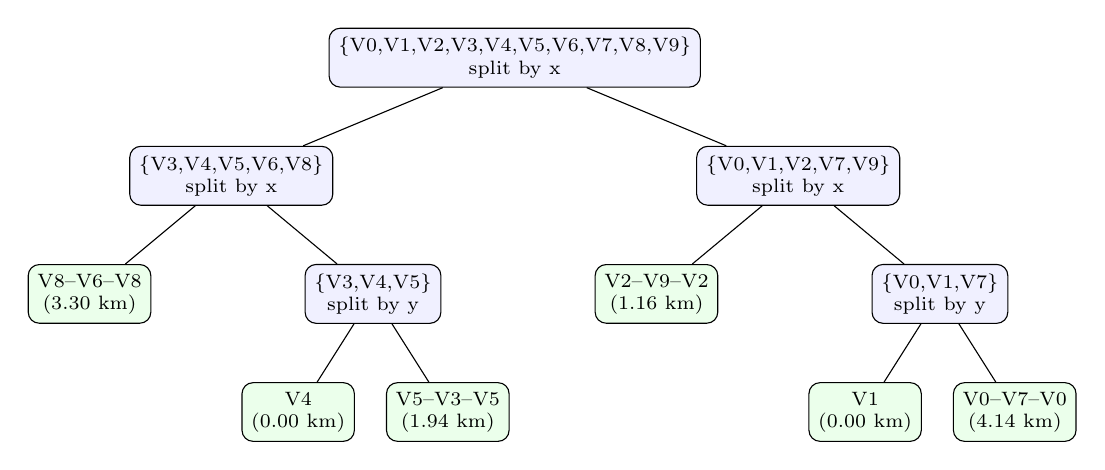
\begin{tikzpicture}[
  split/.style={draw, rounded corners, fill=blue!6, align=center, font=\scriptsize},
  leaf/.style={draw, rounded corners, fill=green!8, align=center, font=\scriptsize},
  level 1/.style={sibling distance=7.2cm, level distance=1.5cm},
  level 2/.style={sibling distance=3.6cm, level distance=1.5cm},
  level 3/.style={sibling distance=1.9cm, level distance=1.5cm}]
\node[split] {\{V0,V1,V2,V3,V4,V5,V6,V7,V8,V9\}\\split by x}
  child {
    node[split] {\{V3,V4,V5,V6,V8\}\\split by x}
    child {
      node[leaf] {V8--\allowbreak V6--\allowbreak V8\\(3.30 km)}
    }
    child {
      node[split] {\{V3,V4,V5\}\\split by y}
      child {
        node[leaf] {V4\\(0.00 km)}
      }
      child {
        node[leaf] {V5--\allowbreak V3--\allowbreak V5\\(1.94 km)}
      }
    }
  }
  child {
    node[split] {\{V0,V1,V2,V7,V9\}\\split by x}
    child {
      node[leaf] {V2--\allowbreak V9--\allowbreak V2\\(1.16 km)}
    }
    child {
      node[split] {\{V0,V1,V7\}\\split by y}
      child {
        node[leaf] {V1\\(0.00 km)}
      }
      child {
        node[leaf] {V0--\allowbreak V7--\allowbreak V0\\(4.14 km)}
      }
    }
  };
\end{tikzpicture}
}
\caption{Divide step for seed \DCSeed{}: recursive median splits by longitude ($x$) or latitude ($y$).
Leaves show the base-case tours and their lengths in km.}\label{fig:tree}
\end{figure}

\paragraph{The same run on the map.} Figure~\ref{fig:steps} draws the recursion on the graph itself.
Panel~(a) shows the median cuts, numbered by recursion level: the level-1 cut is the vertical line that
splits the ten vertices into a western and an eastern half, and the level-2 and level-3 cuts split those
halves again. Panel~(b) shows the base cases: pairs joined by an edge, and single vertices (V1, V4).
Panel~(c)--(e) then undo the cuts from the deepest level up. At each level the sub-tours on the two
sides of a cut are merged by deleting one edge from each (dashed red) and adding the shortest bridge
and a closing edge (gold). After the level-1 merge a single Hamiltonian cycle remains, which is the
final tour. The edge $V_8$--$V_0$ passes visually near $V_2$ in the map, but it is one direct graph
edge; passing near another marker does not visit that vertex or add an extra stop.

\begin{figure}[H]
\centering
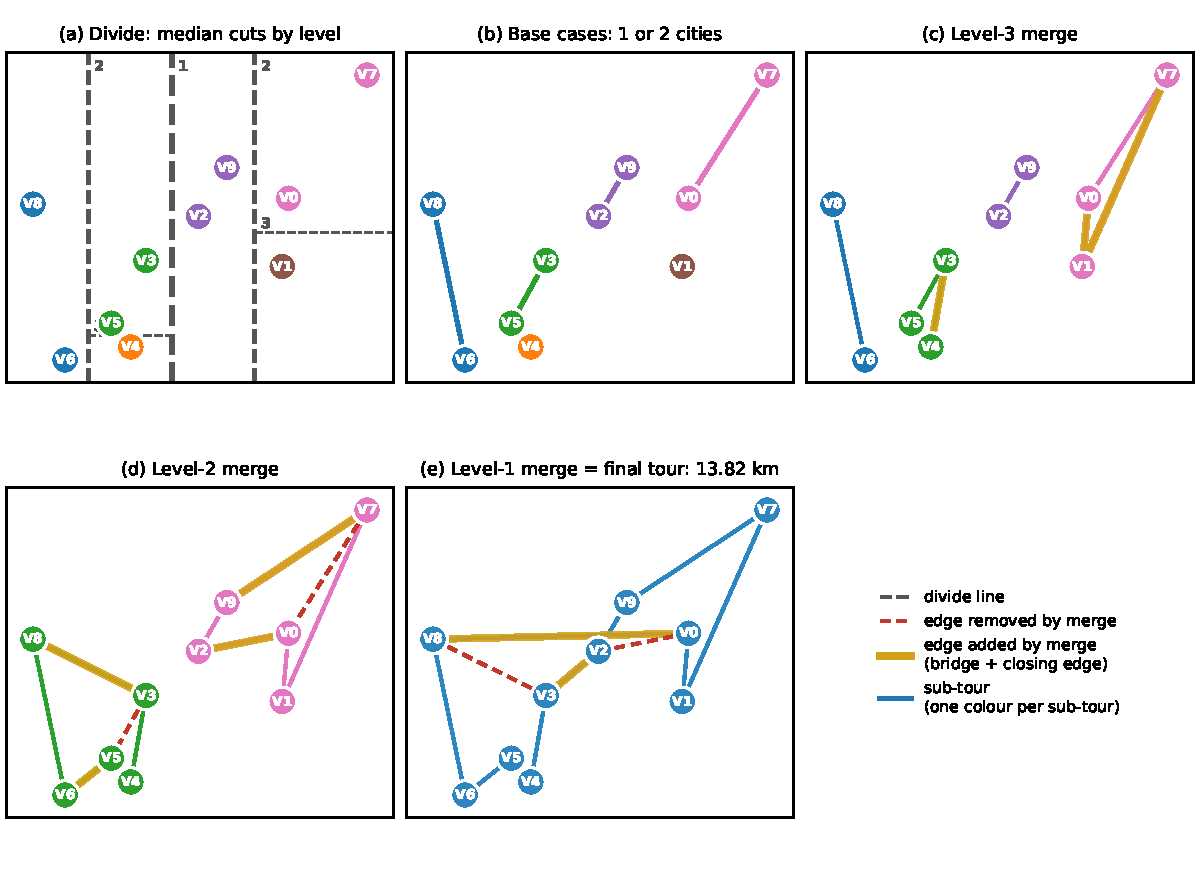
\includegraphics[width=\textwidth]{steps.pdf}
\caption{Divide and Conquer on the graph (seed \DCSeed{}). (a)~Divide lines; (b)~base-case
sub-tours, one colour per sub-tour; (c)--(e)~merges from the deepest level to the top. Dashed red
edges are removed and gold edges are added by a merge. When a two-city tour $a\to b\to a$ is merged,
only one copy of its doubled edge is removed, so that edge stays visible.}\label{fig:steps}
\end{figure}

\paragraph{Conquer and combine.} The sub-tours are merged bottom-up. Table~\ref{tab:trace} lists every
merge: the two input cycles, the shortest bridge, the edges removed and added, the change in length
$\Delta$, and the length of the merged cycle. Each row satisfies
$L(T) = L(T_1) + L(T_2) + \Delta$.

\begin{table}[H]
\centering
\caption{Merge steps (bottom-up). Edge weights in km are given in parentheses.}\label{tab:trace}
\vspace{4pt}
\scriptsize
\setlength{\tabcolsep}{3pt}
% AUTO-GENERATED by code/main.py --export-latex. Do not edit; re-run the export instead.
\begin{tabular}{c >{\raggedright\arraybackslash}p{2.6cm} >{\raggedright\arraybackslash}p{2.6cm} >{\raggedright\arraybackslash}p{1.9cm} >{\raggedright\arraybackslash}p{2.45cm} >{\raggedright\arraybackslash}p{2.45cm} r r}
\toprule
\textbf{Step} & \textbf{Left tour (km)} & \textbf{Right tour (km)} & \textbf{Shortest bridge} & \textbf{Edges removed} & \textbf{Edges added} & $\boldsymbol{\Delta}$ & \textbf{Merged} \\
\midrule
M1 & V4 (0.00) & V5--\allowbreak V3--\allowbreak V5 (1.94) & V4--V5 (0.54) & V5--V3 (0.97) & V4--V3 (1.31), V5--V4 (0.54) & +0.88 & 2.82 \\
M2 & V8--\allowbreak V6--\allowbreak V8 (3.30) & V4--\allowbreak V3--\allowbreak V5--\allowbreak V4 (2.82) & V6--V5 (0.74) & V8--V6 (1.65), V3--V5 (0.97) & V8--V3 (2.15), V5--V6 (0.74) & +0.27 & 6.39 \\
M3 & V1 (0.00) & V0--\allowbreak V7--\allowbreak V0 (4.14) & V1--V0 (1.09) & V0--V7 (2.07) & V1--V7 (2.32), V0--V1 (1.09) & +1.34 & 5.48 \\
M4 & V2--\allowbreak V9--\allowbreak V2 (1.16) & V1--\allowbreak V7--\allowbreak V0--\allowbreak V1 (5.48) & V2--V0 (1.26) & V2--V9 (0.58), V7--V0 (2.07) & V2--V0 (1.26), V7--V9 (1.79) & +0.40 & 7.04 \\
M5 & V6--\allowbreak V8--\allowbreak V3--\allowbreak V4--\allowbreak V5--\allowbreak V6 (6.39) & V9--\allowbreak V2--\allowbreak V0--\allowbreak V1--\allowbreak V7--\allowbreak V9 (7.04) & V3--V2 (1.18) & V8--V3 (2.15), V2--V0 (1.26) & V8--V0 (2.62), V2--V3 (1.18) & +0.39 & 13.82 \\
\bottomrule
\end{tabular}

\end{table}

\paragraph{Worked calculation of the final merge.}
% AUTO-GENERATED by code/main.py --export-latex. Do not edit; re-run the export instead.
The two halves return the sub-tours $T_1 = $ V6--\allowbreak V8--\allowbreak V3--\allowbreak V4--\allowbreak V5--\allowbreak V6 (length 6.39 km) and $T_2 = $ V9--\allowbreak V2--\allowbreak V0--\allowbreak V1--\allowbreak V7--\allowbreak V9 (length 7.04 km).
Checking all $|T_1|\cdot|T_2| = 5\cdot5 = 25$ cross pairs, the shortest bridge is V3--V2 with $w = 1.18$ km.
Among the ways of opening one edge next to each bridge endpoint and closing the loop, the cheapest removes V8--V3 and V2--V0 and adds V8--V0 and V2--V3:
\[\Delta = (2.62 + 1.18) - (2.15 + 1.26) = +0.39\text{ km},\]
\[L(T) = L(T_1) + L(T_2) + \Delta = 6.39 + 7.04 + 0.39 = 13.82\text{ km}.\]
The merged cycle is V3--\allowbreak V4--\allowbreak V5--\allowbreak V6--\allowbreak V8--\allowbreak V0--\allowbreak V1--\allowbreak V7--\allowbreak V9--\allowbreak V2--\allowbreak V3, which visits all 10 vertices once.


Finally, the cycle is rotated to begin at V0, giving the closed route
\begin{center}
\DCRoute{}
\end{center}
of length \textbf{\DCTotal{} km}.
